\setcounter{secnumdepth}{1}

\section{Einführung}

Javascript ist im Aufwind mehr denn je. Sie ist die meist genutzte Programmiersprache unter Entwickler. Laut der jährlichen Umfrage von Stackoverflow im Jahr 2018 belegte sie zum sechsten mal in Folge den ersten Platz.\cite{programming-language-survey} Doch woher kommt dieser Erfolg? \\
Wenn es um das Web geht, war Javascript in der Webentwicklung schon immer Vorreiter. Doch diese Sprache hat seine Stärken auch in der Vielfalt seiner Einsatzmöglichkeiten. Wie mit dem Framework Node.js, dass ab 2009 in Erscheinung getreten ist, war es Möglich Server-seitigen Javascript-Code zu implementieren. Dies hatte zur Folge, dass man sich nicht mit multiplen Programmiersprachen auseinandersetzen musste. Man hatte eine Vereinheitlichung in seiner Code-Basis für seine Applikation gefunden. Zudem bietet Node.js mit npm als Paketmanager die größte Auswahl an Open-Source-Libraries. Ein Weiter Punkt ist die Multi-Plattform-Kompatibilität die Javascript z.B. mit dem Framework React offenbart. Mit diesen Framework ist es Möglich mit einer Code-Basis sowohl Web-Anwendungen als auch Apps auf mobile Geräte zu entwickeln. Da Javascript's Kompilierung vom Betriebssystem unabhängig ist, ist der Übergang von der Webentwicklung zur Mobile-Entwicklung reibungslos. Und genau das bietet auch Typescript. Da Typescript ein sog. \textbf{Superset} von Javascript ist, kann jeder Code von Javascript auch in Typescript interpretiert werden. Der Unterschied zu Typescript und Javascript liegt in ihrer statischen Typisierung. Das bedeutet, dass Variablen, Methoden und Funktionsparameter im Vorfeld mit einem Typ versehen werden. Aufgrund dessen können Bugs am Code schneller erkannt werden. Zudem lässt sich diese Sprache leicht modular aufbauen. Dadurch können Entwicklerteams in Unternehmensprojekte die Code-Struktur besser organisieren und dokumentieren.\\\\

\noindent
Doch mit der Vielfalt steigt auch die Komplexität der Sprache. Besonders da Javascript nicht nur synchron ausführbar ist, sondern auch asynchron. Entwickler bekommen mit dieser Sprache verschiedene Optionen, der asynchronen Datenverarbeitung in Form von Callbacks, Promises und Streams zur Verfügung. Die Einsatzmöglichkeiten können in einem Projekt variieren, jedoch welcher Ansatz in welcher Situation besser geeignet ist, ist besonders für Entwickler mit wenig Erfahrung schwer zu erkennen.


\subsection{Zielsetzung}

Ziel der Arbeit ist die Betrachtung und Aufbereitung des Einsatzes von Sprachmitteln zur asynchronen Verarbeitung in Typescript in einer Form, die Einsteigern in die Thematik hilft, die unterschiedlichen Konzepte voneinander abzugrenzen und richtig einzusetzen. Dazu soll asynchrone Verarbeitung insgesamt anhand brauchbarer und für den Einsatz von Typescript typischer Szenarien motiviert werden. Es werden die zur Verfügung stehenden Sprachmittel Callbacks (im Kurzen), Promises und Observables mit ihren jeweiligen Features vorgestellt. Dabei soll nach dem Vorstellen der Kernkonzepte im zweiten Teil der Arbeit eine Single-Page Applikation mit \glqq Best Practice\grqq{}-Beispiele vorgeführt werden. Nach dem Lesen dieser Arbeit soll der Leser ein gewisses Verständnis dafür gewonnen haben, welche der vorgestellten Sprachmitteln für welchen Anwendungsfall sinnvoller erscheint.\\\\

\noindent
Zielgruppe dieser Arbeit sind Personen, die Grundkenntnisse in der Sprache Javascript/Typescript vorweisen können. Des Weiteren sollte man von den Modell der asynchronen Datenverarbeitung wie Callbacks, Promises und Oberservables schon mal gehört haben, da diese in der Arbeit gegenübergestellt werden.

\subsection{Aufbau}

Diese Bachelorarbeit wird aus zwei Code-Projekten bestehen. Während das erste Projekt nur im Kern die Ausführung von asynchronen Verarbeitungsprozessen präsentiert (mit der Hilfe von simulierten Anwendungsbeispielen), wird das zweite Projekt eine Single-Page Applikation darstellen und praxisnahe Beispiele anwenden. Dies soll mit dem Framework Angular und Google Firebase als DaaS bewerkstelligt werden. Das zweite Projekt wird im zweiten Teil der Arbeit näher vorgestellt. Die Repositories für beide Projekte sind zu finden unter: 

\begin{center}
\url{https://github.com/MarcoLeko/Promises-vs.-Observables.git} \\
\url{https://github.com/MarcoLeko/Angular-Firebase-App.git}
\end{center}

\noindent
Zu beachten ist, dass vor dem Ausführen beider Projekte \textbf{Node.js} auf dem Rechner installiert sein muss, um den integrierten Paket-Manager \textbf{npm} nutzen zu können. Da rxjs nicht von vornherein von Javascript mitgeliefert wird, wird eine sog. \glqq  Third-Party Library\grqq{} dafür benötigt. Daraufhin muss in dem Root-Verzeichnis beider Projekte \textbf{npm install} ausgeführt werden, um die jeweiligen Abhängigkeiten dieser Libraries herunterzuladen. Node.js kann man unter folgendem Link herunterladen:

\begin{center}
\url{https://nodejs.org/en/}
\end{center}

\section{Grundlagen}

Typescript. Bereits der Name sagt schon was diese Sprache ausmacht. Sie \textit{(\glqq{}Type\grqq{} zu deutsch: Typ)} ist eine typisierte Form der Skriptsprache Javascript. Mit dem Typescript Compiler werden Dateien mit dem Suffix *.ts in *.js überführt.

\subsection{Beispiel}

\begin{figure}[H]
\begin{lstlisting}
class Greeter {
    greeting: string;
    constructor (message: string) {
        this.greeting = message;
    }
    greet() {
        return "Hello, " + this.greeting;
    }
}  
\end{lstlisting}
\caption{Typescript Klasse \cite{typescript-example}}
\end{figure}

\noindent
Im oberen Code-Schnipsel wurden die variablen und die Klassenmethoden nach Typescript-Standard deklariert. Diese Typen werden beim übersetzen in Javascript ignoriert. Der Kompiler einer Entwicklungsumgebung prüft dann, ob beim übergeben eines Parameters in den Konstruktor ein numerischer oder Boolean-Wert eingesetzt wird. Dies wird dann als ein Fehler erkannt. Der Kompiler übersetzt auch nicht direkt deklarierte Typen. Wie in diesem Fall wird erkannt, dass die Methode greet() einen String-Wert zurückgibt.

\begin{figure}[H]
\begin{lstlisting}
var Greeter = (function () {
    function Greeter(message) {
        this.greeting = message;
    }
    Greeter.prototype.greet = function () {
        return "Hello, " + this.greeting;
    };
    return Greeter;
})(); 
\end{lstlisting}
\caption{Überführung in Javascript \cite{typescript-example}}
\end{figure}

\noindent
In der vom Kompiler auf Javascript übersetzten Version werden die erstellten Klassen und Typen vollständig eliminiert. Was verbleibt ist die Übersetzung der Klassen-Methode greet() und des Konstruktors. Sowohl Klassen (erst ab ECMAScript2015 verfügbar) als auch Interfaces werden in Javascript nicht genutzt.

\subsection{Kompiler}

In einer tsconfig.json Datei können die Kompiler-Optionen für Typescript gesetzt werden. Zudem können Root-Dateien definiert und ausgeschlossen werden. Die Auflistung einer tsconfig.json Datei in einem Verzeichnis zeigt, dass es sich hierbei um das Root-Verzeichnis des Projekts handelt. Ein Beispiel für die Konfiguration einer solchen Datei könnte wie folgt aussehen: 

\begin{figure}[H]
\begin{lstlisting}
{
  "compilerOptions": {
    "target": "es2018",
    "module": "commonjs",
    "declaration": false,
    "sourceMap": true,
    "noImplicitAny": false,
    "typeRoots": [
      "node_modules/@types"
    ],
    "downlevelIteration": true
  },
  "include": [
    "src/**/*"
  ]
} 
\end{lstlisting}
\caption{Auflistung ist unter der \textbf{tsconfig.json} Datei im Projekt Promises-vs.-Observables zu finden}
\end{figure}

\noindent
Hier kann z.B. mit der Regel \glqq noImplicitAny\grqq{} festgelegt werden, dass Methoden als auch Parameter und Variablen getypt werden müssen bei ihrer Deklaration. Sind sie nicht getypt: Bedeutet dies für den Kompiler sie sind als any deklariert. Kompilefehler.\cite{tsconfig} Zusätzlich ist die Einstellung der Javascript Version möglich. In diesem Fall wird \textbf{EcmaSprict2018} genutzt, dadurch ist die Nutzung neuester Features möglich. Die Konfiguration dieser Datei betrifft nur Fehler beim erstellen eines Kompilats. Fehler zur Laufzeit sind von der Konfiguration ausgeschlossen. Zudem wird in jedem Fall eine Javascript-Datei erstellt, auch wenn der Kompiler einen Fehler anzeigt. Diese Datei ist potenziell auch lauffähig. Um Typescript zu Kompilieren muss im Terminal unter dem Verzeichnis einer Typescript-Datei \textbf{tsc} eingegeben werden. In den für die Bachelorarbeit genutzten Code-Projekte werden die Skripte von npm ausgeführt um die Applikation zu starten. Die Konfiguration eines Start-Skript sieht wie folgt aus:

\begin{figure}[H]
\begin{lstlisting}
  ...
  "scripts": {
    "start": "webpack --watch",
    "build": "webpack"
  }, 
\end{lstlisting}
\caption{Auflistung ist unter der \textbf{package.json} Datei im Projekt Promises-vs.-Observables zu finden}
\end{figure}

\noindent
Wie man hier sehen kann führt \textbf{npm run start} nicht tsc aus, sondern \textbf{webpack --watch} aus. Webpack ist ein sog. \textbf{Module-Loader}. Mit ihm ist es Möglich verschiedene Typescript Klassen/Interfaces/Funktionen aus verschiedene Dateien zu importieren und exportieren. Da Third-Party Libraries in der Applikation genutzt werden, die Klassen und Methoden mitliefern, ist die Nutzung von Module-Loaders unabdingbar. Zudem wird mit Hilfe von Webpack Typescript-Dateien (je nach Konfiguration), inklusive aller involvierten Importe und Exporte, zu einer zentralen Javascript-Datei gebündelt. In der Webpack Konfiguration muss lediglich eine Eingangsdatei definiert werden. Mit der Einstellung --watch werden Veränderung des Codes automatisch erkannt. Das heißt, wenn Änderungen im Code vorgenommen werden, erstellt Webpack ein neues Bündel. Nach dem Kompilieren muss nur noch die HTML-Seite geöffnet werden.\\\\

\noindent
Um mehr von Typescript und z.B. dessen Nutzung mit Module-Loaders zu erfahren, sollte die offizielle Dokumentation von Microsoft durchgegangen werden.

\begin{center}
\url{https://www.typescriptlang.org/docs/home.html} 
\end{center}

\subsection{Terminologie}

Um die Abgrenzung von verschiedenen asynchronen Sprachmitteln zu beherrschen, muss vorerst geklärt werden, was Asynchronität bedeutet.\\\\
\noindent
Der zentrale Teil eines Computers, welches Programme und einzelne Schritte zum Ausführen bringt, ist der Prozessor. Die Geschwindigkeit in der eine Schleife von einem Programm ausgeführt wird, hängt von der Geschwindigkeit des Prozessors ab. Programme interagieren jedoch mit Operationen außerhalb des Zuständigkeitsbereiches eines Prozessors, wie z.B. die Kommunikation über ein Netzwerk oder Abfragen von Daten von der Festplatte. Solche Operationen hängen von anderen Ressourcen ab und brauchen Zeit. In solchen Szenarien wäre es unvorteilhaft, wenn der Prozessor, anstatt andere Operationen in der Zwischenzeit auszuführen, im Leerlauf stecken würde. Genau für solche Aufgaben ist das Betriebssystem da. Das Betriebssystem sorgt dafür, dass Kapazitäten des Prozessors auf parallel laufende Programme wechselt, während es auf die Antwort von ausgeführten Operationen wartet. Es entstehen dabei verschiedene \glqq Threads\grqq{}. Und hier kommt die Asynchronität ins Spiel:

\subsubsection{Asynchronität}

Ein \textbf{asynchrones} Programmiermodell erlaubt multiple Abläufe zum selben Zeitpunkt. Wenn eine Aktion ausgeführt wird, läuft das Programm in einem anderen \glqq Thread\grqq{} weiter. Sollte die Operation fertig gestellt sein, wird das Programm informiert und liefert das Ergebnis zurück. Ein Beispiel dafür wäre das Suchen von Dateien auf einer Festplatte.\cite{asynchronitaet} \\

\subsubsection{Synchronität}

In einem \textbf{synchronen} Programmiermodell entstehen Abläufe sequenziell. Wenn eine Funktion mit einer zeitintensiven Aktion abgerufen wird, wird das Ergebnis erst nach dem Beenden der Operation zurückgegeben. In diesem Zeitintervall werden keine Nebenoperationen ausgeführt.\cite{asynchronitaet} \\

\subsubsection{Beispiel}

Die Wiedergabe mehrerer Meldungen in einem Browser. Vor dem Ausführen des Beispiels muss folgend konfiguriert werden:

\begin{center}
    Promises-vs.-Observables$\,\to\,$ webpack.config.js
\end{center}

\begin{figure}[H]
\begin{lstlisting}
module.exports = {
    mode: 'development',
    entry: './src/modules/sync-vs-async.ts',
    ...
}
\end{lstlisting}
\caption{Hier sollte vor dem Starten des Projekts die Typescript Datei sync-vs-async.ts als Eingangspunkt definiert werden.}
\end{figure}

\begin{figure}[H]
\begin{lstlisting}
export class Print {

    public msg(msg: string): void {
        document.body.innerHTML +=
            `<div class="alert" role="alert">${msg}</div>` as string;
    }

    public time(begin: number, end: number, css: string) {
        document.body.innerHTML += `<div class="time-box ${css}">time: ${end - begin}ms</div>`;
    }
}
\end{lstlisting}
\end{figure}

\begin{figure}[H]
\begin{lstlisting}
class Synchronous extends Print {

    public printAndTrackTime() {
        const begin = window.performance.now();
        this.printMessages();
        const end = window.performance.now();
        this.time(begin, end, 'sync');
    }

    private printMessages(): void {
        this.msg('Hey Im message Nr. 1!');
        this.msg('Hey Im message Nr. 2 !');
        this.msg('Hey Im message Nr. 3 !');
    }
}

class Asynchronous extends Print {

    public printAndTrackTime() {
        const begin = window.performance.now();
        this.printMessages();
        const end = window.performance.now();
        this.time(begin, end, 'async');
    }

    private printMessages(): void {
        this.msg('Hey Im message Nr. 1 !');
        setTimeout(() => this.msg('Hey Im message Nr. 2 !'), 50);
        this.msg('Hey Im message Nr. 3!');
    }
}
\end{lstlisting}
\end{figure}

\begin{figure}[H]
\begin{lstlisting}
const sync = new Synchronous();
const async = new Asynchronous();

sync.printAndTrackTime();
document.body.innerHTML += '<hr>';
async.printAndTrackTime();
\end{lstlisting}
\caption{sync-vs.-async.ts}
\end{figure}

\noindent
Diese Datei enthält drei Klassen. Während \textbf{Print} als Basisklasse eine Methode für das Addieren einer Nachricht in die HTML-Dom bereitstellt, rufen die abgeleiteten Klassen \textbf{Synchronous} und \textbf{Asynchronous} die Nachricht in verschiedener Weise auf. In der Klasse Synchronous werden die HTML-Elemente sequenziell in die Dom eingefügt. In der Asynchronous Klasse dagegen wird nur die erste und dritte Nachricht sequenziell ausgeführt. Die zweite Nachricht wird mit einer Verzögerung von 50 Millisekunden in einem neuen Zeitfenster veranlasst. Ein neuer Thread entsteht. Währenddessen wird schon die nächste Operation ausgeführt. Um die Zeit zurückzuverfolgen wurde ein Timer vor der Anzeige der HTML-Elemente gestartet. Dieser wird gestoppt sobald alle Nachrichten innerhalb dieser Methode aufgerufen wurden. Auffallend ist, dass die Methode in der synchronen Ausführung stets länger braucht als die asynchrone Ausführung. Das liegt daran, dass in der asynchronen Ausführung die Zeit nach dem Ausführen der dritten Nachricht und vor dem Ausführen der zweiten Nachricht gestoppt wird, da die zweite Nachricht sich in einem anderen Zeitfenster befindet. Somit wartet der Timer im asynchronen Modell immer nur auf zwei Nachrichten, während das synchrone Modell auf drei Nachrichten wartet.
Das Ergebnis sieht wie folgt aus:

\begin{figure}[H]
\centering
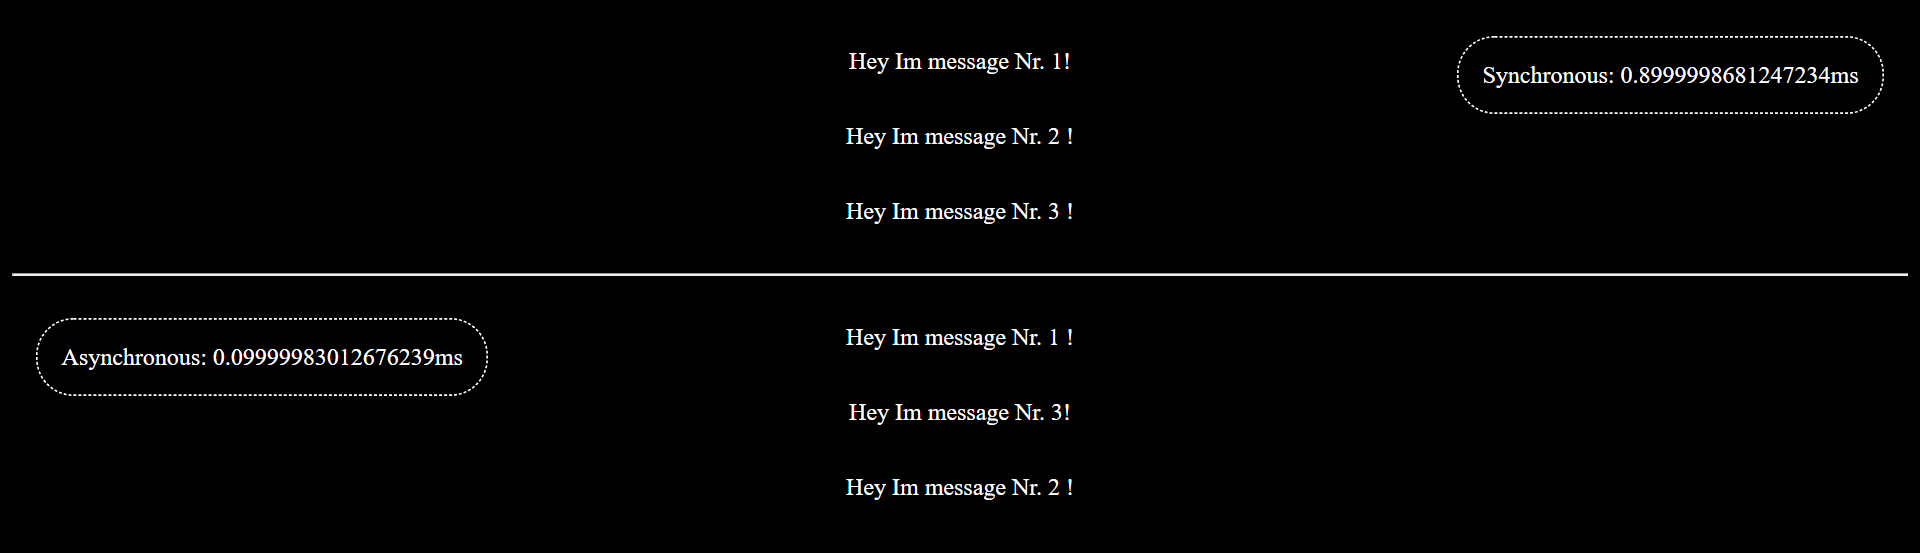
\includegraphics[width=12cm, height=6cm]{synchronous-vs-asynchronous}
\caption{Die Asynchronous Klasse gibt Nachricht 3 aus bevor Nachricht 2 ausgegeben wird.}
\end{figure}

\noindent
Zusammenfassend kann man also sagen, dass in dem synchronen Modell implizit auf die Aktionen gewartet wird, und in dem asynchronen Modell explizit. Als Diagramm abgebildet führt der Browser die Methoden wie folgt aus:

\begin{center}
\begin{figure}[H]
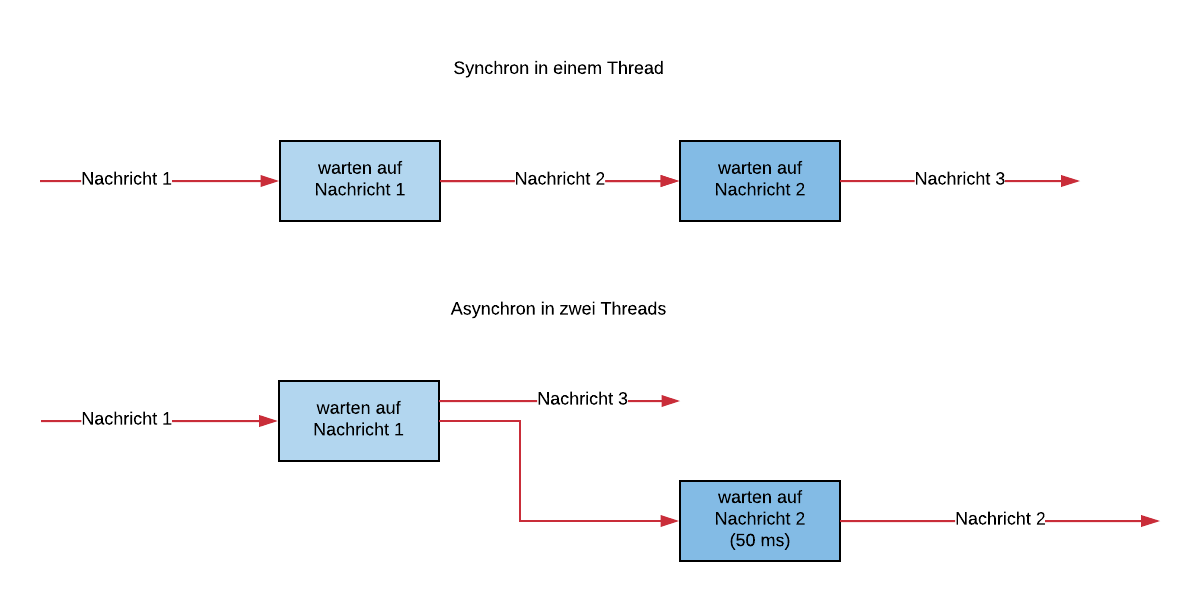
\includegraphics[width=12cm]{synchron-vs-asynchron-diagramm}
\caption{Ablauf der ausgeführten Operationen im Browser}
\end{figure}
\end{center}

\noindent
Das angeführte Beispiel hat mit der Funktion setTimeout eine asynchrone Operation ausgeführt. Funktionen die als Parameter andere Funktionen übergeben werden, nennt man auch \textbf{Callback function} - Rückruffunktionen. Es gibt jedoch auch andere Ansätze der asynchronen Prozessverarbeitung.





